%  !TEX root = ../main.tex

\section{Evaluation}
\subsection{Experiment Setup}
\subsubsection{Overview} We implement \alias using PyTorch~\cite{pytorch} on a Ubuntu 20.04 server with Intel Xeon 6226R 2.90GHz CPU and NVIDIA 3090 GPU. Based on our experiments, we empirically set the default configuration as $\delta=1.2s$, $\xi=5s$, $\epsilon=1$, $0.5\le\beta\le1.5$, sync range $T$=100~ms, $maxEpoch$=800. Adam optimizer~\cite{kingma2014adam} is used to speed up our convergence.
For evaluating \alias's effectiveness in fooling ASR while users use it, we select the end-to-end DeepSpeech2~\cite{amodei2016deep} as the target model and conduct experiments in both digital and physical scenarios.

\subsubsection{Dataset}\label{sec:eval_dataset} We adopt the typical Fluent Speech Command Dataset~\cite{fluent2020commands} to examine the effectiveness of \alias, including 30,046 voice command samples. 
We randomly selected 896 samples from the 10-person validation set given in the dataset, with each speaker contributing around 90 utterances on average. These samples are used to craft our perturbation. The remaining unseen 29,150 samples are used to evaluate \alias under various settings. % And we conduct testing on 29,150 commands which are unseen to \alias.

\subsubsection{Hardware} We employ a signal generator (SIGLENT SDG6032X)~\cite{siglent} to modulate the created IAPs, a power amplifier (NF HSA4015)~\cite{amplifierHSA4015} to enable long-range delivery, and a custom ultrasound transducer array to emit the modulated IAPs. The recording devices to be tested include Google Pixel 3aXL, iPhone14 pro, MI Mix2s, OPPO Reno5 pro, and ReSpeaker Mic array v2.0~\cite{respeaker}, where all model versions are released in the last five years. Moreover, we evaluate attacks with a self-made portable device and a loudspeaker in \textsection\ref{sec:portable_attack}.

% https://tutorials.hybrik.com/analyze_audio_psnr/ PSNR and SNR
\subsubsection{Metrics} (1) We use the success rate (SR) to indicate the percentage of \alias successfully altering user commands and matching target transcriptions in all attempts. (2) We use character error rate (CER), a representative metric in ASR tasks, to indicate the adversary's ability to tamper with user commands from the character level; a lower CER represents a more effective attack. (3) Signal-to-Noise Ratio (SNR) and $L2$-distortion are vital for audible-band AEs because of the imperceptibility requirements. SNR: the ratio of benign audio power to the perturbation power. $L2$: the sum of squared amplitude. AEs with a low SNR and high $L2$ are more likely to be noticed, and vice versa.

\subsection{Digital Attack Performance}
As our attack focuses on real-world scenarios, where physical disturbances always exist, we incorporate the effects of physical conditions by employing our ultrasonic transformation modeling to guarantee that digital attack performance has physical significance. % We collect 15 UFRs and noises from different angles at the same distance for generating the universal perturbations.

\subsubsection{Impact of Optimization Space} %$\epsilon$
Since the delivery of \alias is inaudible, it facilitates the unconstrained advantage of setting $\epsilon$ up to $1$ (i.e., the normalized audio's upper bound) for universal attacks. We further explore attack capability under different $\epsilon$ upper bounds, both universal and silence IAPs.
We optimize silence perturbations according to $\epsilon=0.2, 0.4, 0.6, 0.8, 1.0$, respectively, aiming to tamper the user instructions to the blank. In addition, we obtain the universal perturbations expected to alter user commands to ``open the door'' with the same settings. CTC loss convergence curves are shown in Fig.~\ref{fig:dig_exp1}. We observe that the crafting process can converge faster as the $\epsilon$ (i.e., the optimization space) increases in both tasks. After $\epsilon$ reaches $0.8$, the convergence rate approaches the maximum.
Then we estimate the physical delivery of both perturbations via an unseen transformation model (i.e., a pair of UFR and anomalous noise not involved in training). The transformed perturbations are further superimposed on every test voice command sample. Results listed in Tab.~\ref{tab:dig_exp1} show that, in addition to the faster convergence, a larger $\epsilon$ significantly boosts the universality of \alias. It can successfully alter 18,946 samples into ``open the door'' and mute 27,531 user commands into blank `` '', which highlights \alias features a highly universal capability.  % exceeds 50 commands denied by an AE in previous work~\cite{guo2022specpatch}.


\begin{figure}[!t]
        % \vspace{-7pt}
	\centering  %居中
        \subfigure[Silence Perturbation]{   %第一张子图
    	\begin{minipage}[t]{0.225\textwidth}
    		\centering
                % \hspace{-0.25\linewidth}
    		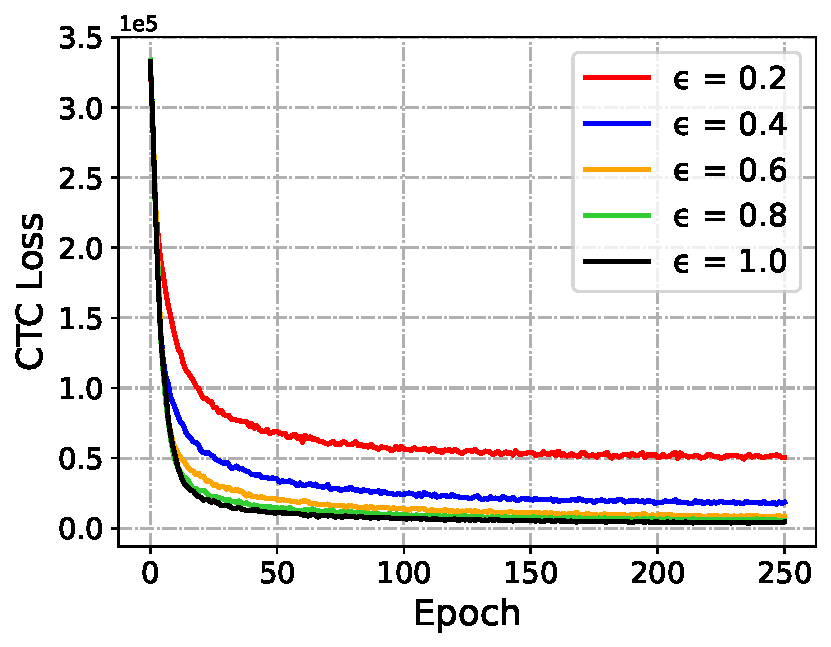
\includegraphics[width=1\textwidth]{exp1_mute_attack.pdf} % height=0.765\linewidth
    	\end{minipage}
        }
	\subfigure[Universal Perturbation]{   %第一张子图
	\begin{minipage}[t]{0.225\textwidth}
		\centering
            \hspace{-0.1\linewidth}
		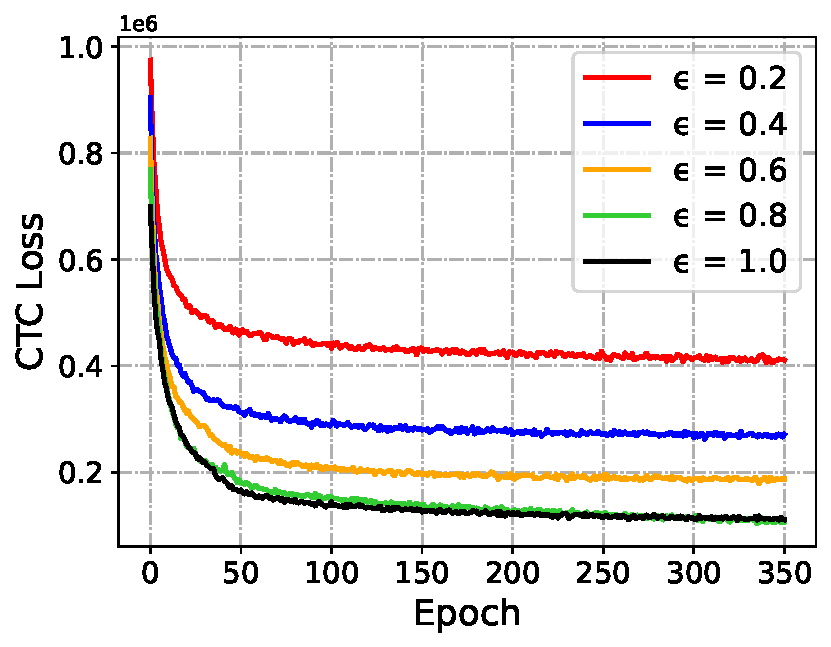
\includegraphics[width=1\textwidth]{exp1_uni_attack.pdf} 
	\end{minipage}
	}
	\caption{CTC loss curves of silence and universal perturbations during the optimization process under varying $\epsilon$.}    %大图名称
	\label{fig:dig_exp1}    %图片引用标记
	\vspace{-10pt}
\end{figure}

\begin{table}[t]\footnotesize
	\centering
		\caption{The number of successfully silenced/altered test speech samples under different $\epsilon$ upper bounds}
		% \vspace{-8pt}
		%	\setlength{\abovecaptionskip}{0in} 
		%	\setlength{\belowcaptionskip}{0in}
		\renewcommand\arraystretch{0.8}
		\renewcommand\tabcolsep{5pt}
		\begin{threeparttable}
			\begin{tabular}{c|c|c|c|c|c}
				\toprule
				\textbf{Upper Bound ($\epsilon$) } & \textbf{$0.2$} & \textbf{$0.4$} & \textbf{$0.6$} & \textbf{$0.8$} & \textbf{$1.0$} \\
				\midrule
				\textbf{Silence Perturb.} & 1,591 & 8,095 & 17,064 & 24,832 & 27,531 \\ \midrule
				\textbf{Universal Perturb.} & 649 & 5,268 & 13,085 & 16,726 & 18,946 \\
				%			\midrule
				\bottomrule
			\end{tabular}
		% \vspace{-10pt}
		\end{threeparttable}
		\label{tab:dig_exp1}
\end{table}


\subsubsection{Comparison of Convergence Overhead and Audibility Cost for the Universality Goal}\label{eval:dig_compare} % CW imperceptible specpatch ours
\blue{The unconstrained advantage of \alias ($\epsilon=1$) empowers its high universality. We further compare it with 3 classical audible-band AEs (i.e., CW~\cite{carlini2018audio}, Qin~\cite{qin2019imperceptible}, and SpecPatch~\cite{guo2022specpatch}) regarding the cost for achieving the same universality goal of each method. We reproduce these works strictly following their instructions.
We set \textit{two goals}: creating a single perturbation that can alter 1) one or 2) five commands based on each method. Notably, for audible-band AEs, we employ RIRs for physical simulation to be consistent with our default setup.
We specify the minimal upper bounds $\epsilon$ of CW, Qin, and SpecPatch to $0.03,0.05,0.05$, respectively, based on which the three methods can maintain universality for 5 commands, i.e., finally converge to the target transcript ``Open the door''. 
We examine also the CTC loss convergence speed of 4 methods. The normalized loss curves in Fig.~\ref{fig:dig_exp2} clearly show that \alias (in red) converges within the fewest iterations among 4 methods; SpecPatch (in blue) converges slowest as it is devised to be short (0.5s). Specifically, we list the overall duration for each methods to final convergence for altering 5 commands---\alias: 1.63~min, CW: 6.52~min, Qin: 9.16~min, and SpecPatch: 35.38~min. \alias converges faster because (1) we reduce optimization complexity by only picking 5 random UFR/noise pairs rather than all ultrasonic channel data per iteration; (2) \alias can quickly find feasible solutions due to its broad optimization space.}
In addition, Tab.~\ref{tab:dig_exp2} demonstrates the SNRs and $L2$-distortion values of audible-band AEs under different universality goals. All SNRs of these AEs are low due to a compromise of physical robustness and imperceptibility, with the highest SNR down to 22 dB. Moreover, if the goal number increases, audible-band AEs are bound to get louder and more easily heard.


\begin{figure}[t]
  \centering
  \begin{minipage}[b]{0.235\textwidth}
    \centering
    \hspace{-0.1\linewidth}
    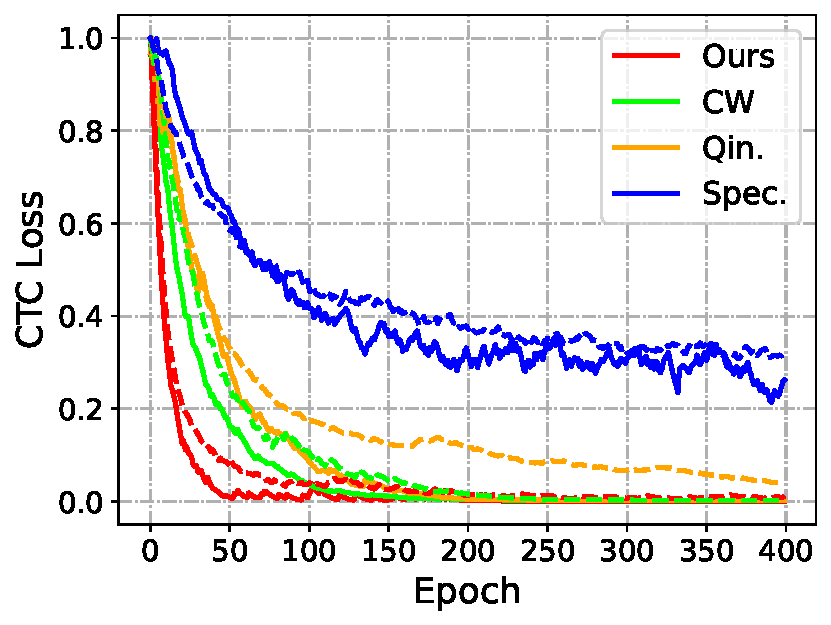
\includegraphics[width=\textwidth]{exp2_compare_attack.pdf}
  \end{minipage}
  \hfill
  \begin{minipage}[b]{0.235\textwidth}
    \centering
    \footnotesize
    \renewcommand\arraystretch{0.7}
    \renewcommand\tabcolsep{2.pt}
    \hspace{-0.1\linewidth}
    \captionof{table}{Audibility cost}\vspace{-10pt}
    \raisebox{0.35\linewidth}{
        \begin{tabular}{c|c|c|c}
            \toprule
            \textbf{Method~} & \textbf{~Goal~} & \textbf{~~SNR~~}  & \boldmath{~~$L2$~~} \\ \midrule
            \multirow{2}{*}{CW}    & 1    & 22dB & 1.31 \\ & 5    & 18dB & 2.24 \\ \midrule % ~\footnotesize{($\epsilon$:0.03)}
            \multirow{2}{*}{Qin}   & 1    & 22dB   & 1.42 \\ & 5  & 17dB   & 2.67 \\ \midrule % ~\footnotesize{($\epsilon$:0.05)}
            \multirow{2}{*}{Spec.} & 1    & 8.5dB  & 122 \\ & 5   & 8.4dB   & 123 \\ \bottomrule % ~\footnotesize{($\epsilon$:0.05)}
        \end{tabular}
        \label{tab:dig_exp2}
    }
  \end{minipage}
  \normalsize
  \caption{CTC loss curves. Compare the convergence speed of \alias with 3 classical audible-band AEs. Dashed lines: train a perturbation that can simultaneously alter 5 voice commands; likewise, Solid lines: alter 1 command, thus converging faster than the former.}
  \label{fig:dig_exp2}
  \vspace{-12pt}  
\end{figure}


\subsubsection{Different Target Commands}\label{sec:eval_commands}
% 我们根据
Given that adversaries may launch attacks for various purposes, they will craft different adversarial perturbations accordingly.
In this experiment, we first train 10 universal perturbations referring to typical malicious commands~\cite{petracca2015audroid} listed in Appendix \textsection\ref{append:command_list} Tab.~\ref{tab:diff_commands} along with the silence perturbation. Then we apply \alias to 7,200 benign commands to validate its effectiveness, amounting to 72,000 samples. 
We count the success rate when transcription outputs match the target commands correctly. In addition, we also count CERs over all samples. We find no significant performance varying with target transcripts, where most targets derive a 100\% SR and 0\% CER (7 out of 10). The lowest SR is still up to 92.82\%, corresponding to ``Mute volume and turn off the WiFi''. Moreover, it is worth noting that the highest CER of these targets is still down to 0.50\%, suggesting \alias can tamper with user commands well from the character level. Due to page limitations, the details are listed in Appendix~\ref{append:command_list} Tab.~\ref{tab:diff_commands}.

\subsection{Physical Attack Performance}
We perform extensive physical experiments to evaluate the practical performance of \alias under different conditions, i.e., w/o our modeling, distances, environments, recording devices, etc.
In the physical experiments, %we use the same universal and silence perturbations evaluated in digital attacks.
we set the target intent as ``open the door'', the attack distance 4m away from the recording devices with the injection angle pointing to their bottom microphones as the default configuration unless otherwise specified. Except for the experiments about different scenes, the rest are conducted in a laboratory of approximately 13.6m$\times$5.2m with slight HVAC noises. We employ a custom ultrasonic transmitter for inaudible adversarial perturbation delivery. A loudspeaker plays the audible benign speech samples, and the ambient noise level is around 38~dB. 
\blue{We also deploy a VAD-based program in conjunction with a microphone connected to the laptop to trigger IAPs delivery using the synchronization-aided design. This ensures real-time triggering when audible benign speech initiates.}
Our real-world attack scenario is given in Appendix \textsection\ref{append:attack_scenario}, Fig.~\ref{fig:attack_actual}. 
Due to page limitations, we elaborate on the impact of angles in Appendix \textsection\ref{append:eval_angles}.

\subsubsection{Ablation Experiments w/o Transformation Modeling}\label{sec:eval_utm}
To validate the effectiveness of our ultrasonic transformation modeling, we apply 3 strategies to craft IAPs. In addition, we apply direct ultrasound-based attacks as the baseline group (\textit{G1}).
The first strategy is an optimization without transformation, i.e., $h_{\theta}(d)\ast\delta+n$ in Eq.~\ref{equ:sync_attack} is degraded to simple $\delta$ during the crafting process (\textit{G2}). 
Similarly, the second strategy uses a low-pass filter, reducing the precise transformation to a filter that allows signal components below 3~kHz to pass (\textit{G3}).
The third strategy is crafting a perturbation with \emph{our transformation}, i.e., \alias (\textit{G4}). 
We carry out experiments with synchronization-aided emission of both benign audio and attacks. We select 40 benign utterances to be played via loudspeaker, and finally collect 480 mixed samples (120 per group) by repeating the operation three times for minimizing errors. Tab.~\ref{tab:wo_transformation} lists each group's success rate and average CER, which remarkably denotes that our modeling can well describe the digital-to-physical transformation during optimization. Approximating the transformation as a low-pass filter can also generate a physically available perturbation with 21.67\% SR and 19.39\% CER. The attack performance decreases to 0\% in \textit{G1} and \textit{G2}. However, attacks without modeling still outperform the baseline (\textit{G1}) from the CER perspective due to leveraging the model vulnerability.


\begin{table}[t]\footnotesize
	\centering
		\caption{Ablation of w/o transformation modeling}
		\renewcommand\arraystretch{0.7}
		\renewcommand\tabcolsep{2pt}
		\begin{threeparttable}
			\begin{tabular}{c|c|c|c|c}
				\toprule
				\textbf{Metrics} & \textbf{Baseline (\textit{G1})} & \textbf{Without (\textit{G2})} & \textbf{Low-pass (\textit{G3})} & \textbf{With (\textit{G4})} \\
				\midrule
				\textbf{SR} & 0\% (0/120) & 0\% (0/120) & 21.67\% (26/120) & 100\% (120/120) \\ \midrule
				\textbf{CER} & 95.7\% & 78.93\% & 19.39\% & 0\% \\
				%			\midrule
				\bottomrule
			\end{tabular}
		\end{threeparttable}
		\label{tab:wo_transformation}
\end{table}

\begin{figure}[t]
    \centering
    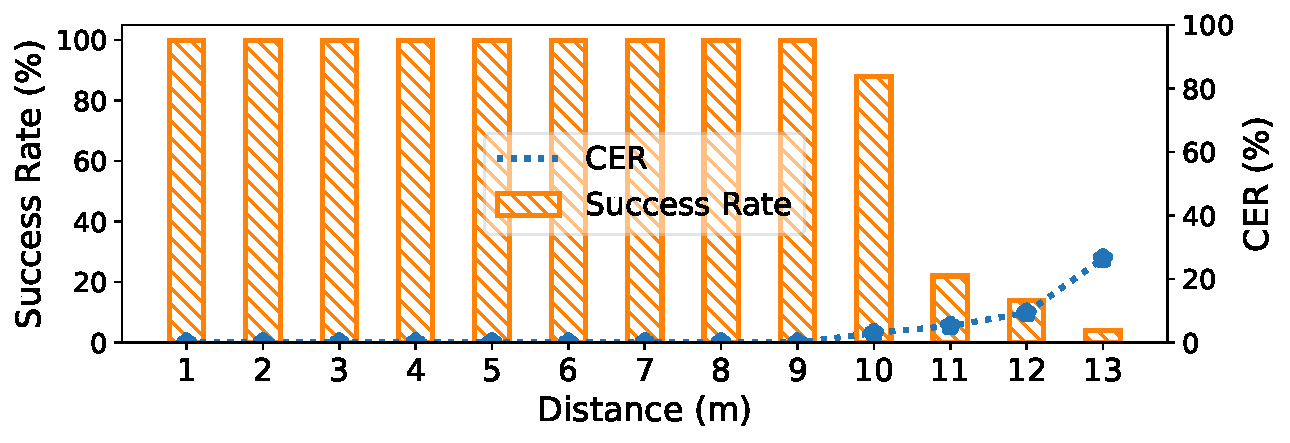
\includegraphics[width=0.45\textwidth]{attack_distance.pdf}
    \caption{\alias's performance at different distances.}
    \label{fig:attack_distance}
    \vspace{-10pt}
\end{figure}
\subsubsection{Different Attack Distances}
% 探究不同攻击角度和距离对于结果的影响
Attacks in the audible band are constrained by concealment, resulting in perturbations that cannot be delivered with more extensive ranges. By contrast, our attack delivery via ultrasound modulation can apply substantial power, which overcomes the attenuation nature of ultrasound. We adjust the amplifier gain so that the high-frequency beam's energy reaching microphones is maintained, thus ensuring the effectiveness of \alias. Specifically, we conduct experiments at the ultrasonic transmitter away from the receiving device within 1m$\sim$13m (1m interval), where the maximum power at 10m$\sim$13m is approximately 3.2 Watt. We randomly select 40 voice commands and play them at each location. We repeat the perturbation superimposed on the benign command 3 times and totally collect 1,560 samples, with 120 per distance, respectively, as well as feed them into the ASR model. We count the success rate and CER in Fig.~\ref{fig:attack_distance}, where \alias is very effective within 1m$\sim$9m as the SRs are up to 100\% and CERs are down to 0\%. The SR is 88.7\% and CER is still down to 3.25\% at 10m. Besides, we observe the attack performance decrease at 11m$\sim$13m. We believe this is due to the ultrasound attenuation, which makes the perturbation less significant to the ASR model. We also discuss this issue in \textsection\ref{sec:discuss}.

\begin{table}[t]\footnotesize
	\centering
		\caption{Different attack scenes}
		% \vspace{-8pt}
		%	\setlength{\abovecaptionskip}{0in} 
		%	\setlength{\belowcaptionskip}{0in}
		\renewcommand\arraystretch{0.7}
		\renewcommand\tabcolsep{3pt}
		\begin{threeparttable}
			\begin{tabular}{c|c|c|c|c}
				\toprule
				\textbf{Scene} & \textbf{Office} & \textbf{Lounge} & \textbf{Laboratory} & \textbf{Corridor} \\
				\midrule
				\textbf{SR} & 100\% (40/40) & 95\% (38/40) & 100\% (40/40) & 92.5\% (37/40) \\ \midrule
				\textbf{CER} & 0\% & 0.79\% & 0\% & 1.04\% \\
				%			\midrule
				\bottomrule
			\end{tabular}
		% \vspace{-10pt}
		\end{threeparttable}
		\label{tab:diff_scene}
\end{table}

% We are able to show to some extent that our modeling overcomes the problem of position dependence. Showing the validity of our consideration of location in modeling


\subsubsection{Different Scenes}
% 探究不同大小的房间中实施攻击
To examine the effectiveness of \alias in different environments, our experiments include a small office (2.4m$\times$2.6m, 36~dB), medium lounge (6.3m$\times$3.8m, 42~dB), large laboratory (13m$\times$5.2m, 38~dB), and narrow corridor (60m$\times$2m, 44~dB). In these scenes, the reverberation pattern of audible sound varies with space size.
Our configuration consists of a transmitter-to-device distance of 4m and a loudspeaker-to-device distance of 1m, which mimics the standard user interaction distance, except the distance of 2.5m for the small office due to its limited size. 
We also play 40 audible benign samples and superimpose \alias on them for once. Then we collected 160 samples from 4 spaces. As shown in Tab.~\ref{tab:diff_scene}, we find no significant difference between these scenarios, as our design considers such physical variation.

\begin{figure}[t]
    \centering
    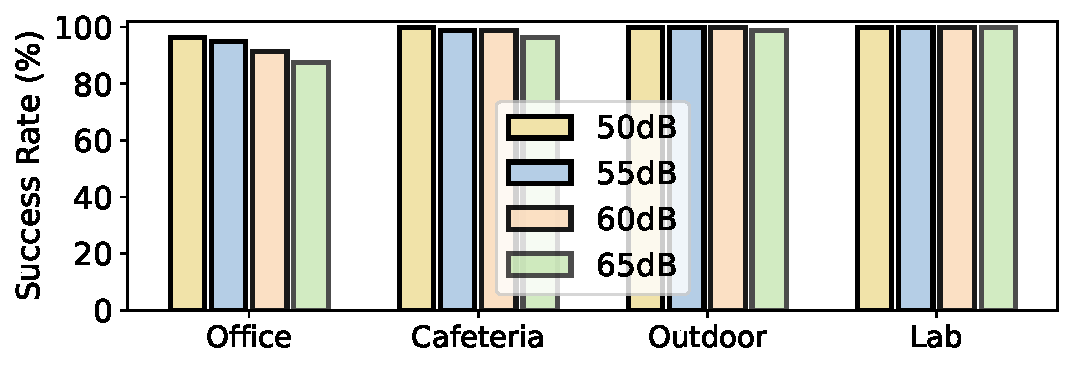
\includegraphics[width=0.42\textwidth]{eval_noises.pdf}
    \caption{Attack performance in face of noises from typical scenes at 4 sound pressure levels.}
    \label{fig:eval_noises}
    \vspace{-10pt}
\end{figure}

% In the small office, there is the sound of people talking and communicating (cafe, keyboard), in the break room there is the sound of TV programs playing (show), in the large lab there is the workstation sound (bedfan), and long and narrow corridor scenes (60m*2m). 
\subsubsection{Different Ambient Noises}
We perform ambient noise-related experiments in our laboratory, where noises of 4 typical scenes are involved, i.e., cafeteria (people chatting), office (keyboard typing), lab (machine running), and outdoor (wind blowing) downloaded from the freesound~\cite{freesound}.
We evaluate noise starting from 50$\sim$65~dB, with 5~dB intervals, and we play noises through an additional loudspeaker to guarantee the noise pressure level reaches the receiver at 50, 55, 60, and 65 dB. Noise samples from 4 scenes are played continuously. At the same time, we play 20 audible benign commands and deliver \alias. Given that the noise is not constant, the superposition of different parts may have different effects. We repeat the above operation three times and collect 240 mixed samples for each noise level. Fig.~\ref{fig:eval_noises} demonstrates that \alias maintains effectiveness even if the noisy ambient sound reaches 65~dB with an average SR up to 97.65\%. The performance drops slightly in the office noise case of 87.5\%, where the keyboard typing and mouse striking are crisp noises with intense high-frequency energy. Since \alias mainly affects low-frequency acoustic features after transformation, high-frequency noise might reduce its attack performance on deceiving ASR models. 

\begin{figure}[t]
    \centering
    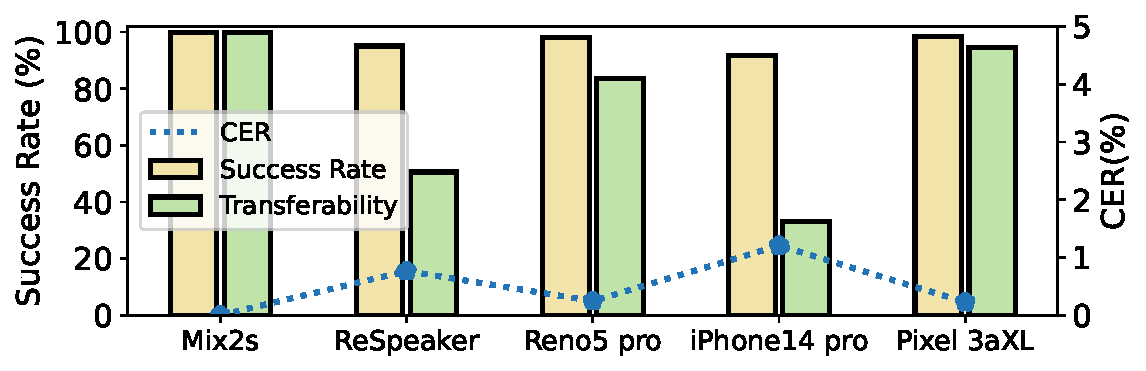
\includegraphics[width=0.42\textwidth]{phy_phones.pdf}
    \caption{Attack performance on different recording devices.}
    \label{fig:phy_devices}
    \vspace{-10pt}
\end{figure}

\subsubsection{Different Recording Devices}
Since the ultrasound frequency response varies with different recording devices and microphone models~\cite{li2023learning}, i.e., we establish a specific transformation model for each device.
To verify that our perturbation can still manipulate the ASR model after being recorded by different devices, we obtain 5 pairs of universal and silence perturbations based on the device-wise ultrasonic transformation. 
After a similar collection as the above experiments done for each device, Fig.~\ref{fig:phy_devices} depicts the average SR of these devices is up to 96.8\% and CER is down to 0.50\%, where Mix2s reaches 100\% and 0\% on these metrics, proving the crafted \alias's effectiveness on individual devices. Moreover, \alias gets 95.8\% SR on ReSpeaker, suggesting it can also attack devices with multi-channel microphones well.
\blue{
Furthermore, given that adversaries may attack unmodeled (i.e., unseen) devices, we want to investigate \alias's transferability despite our ultrasound transformation modeling is device-specific. We apply the optimized perturbation of Mix2s to other devices. Among them, the Mix2s' combined perturbation can transfer to Pixel 3aXL and Reno5 pro with 94.2\% and 83.3\% SR. Besides, the performance reduces on iPhone14 pro (31.7\%) and ReSpeaker (50.8\%) due to their microphones' different frequency selectivity to ultrasound. The result indicates that \alias is also transferable across devices.}

\subsubsection{Different Speech \& Perturbation Loudness}
We further investigate the attack performance changes due to different loudness of the user speech and the universal perturbation. 
We set the representative audible sound pressure level to vary from 65$\sim$90~dB using a decibel meter and also vary ultrasonic emission power to keep the same loudness.
We play our perturbation, repeating 5 times at each volume level. Due to page limitation, results are given in Appendix \textsection\ref{append:loudness_compare}, Fig.~\ref{fig:loudness_compare}. As the mutual loudness changes, we find that once the perturbation has the same volume as the benign audio, it achieves over 55\% SR.
Moreover, with 5~dB higher than the benign audio, \alias can work effectively with an average SR up to 95.5\%. When \alias's volume is 10~dB higher than audible speech, it can dominate all the user commands. Notably, even if the direct ultrasound-based attack is 35~dB louder than the audible audio, the ASR model still recognizes a CER up to 46\%. In that case, \alias achieves all CERs down to 0\%.

\subsection{Attack with Portable Device and Off-the-shelf Loudspeaker}\label{sec:portable_attack}
Our sophisticated device facilities an extensive attack range, providing great flexibility to attackers. We have also implemented two other covert attacks with the portable device and everyday life loudspeaker, as shown in Fig.~\ref{fig:portable_device}.
\subsubsection{Portable Device}
Our portable device equipped with eight 25~kHz ultrasound transducers, a compact amplifier, and a rechargeable battery in Fig.~\ref{fig:portable_device}(a), balances lightweight and attack range. It can be connected to the smartphone, where the attacker stores perturbations as 96~kHz USB-AM audio in advance. We evaluate the effectiveness of attacks with a portable device, setting it to point at Mix2s' bottom microphone with the target ``open the door''. Fig.~\ref{fig:eval_portable_hivi}(a) demonstrates 100\% SR within 150~cm, and 78\% SR along with CER down to 1.69\% even at a distance of 180~cm, suggesting \alias with portable devices can exceed the attack distance of almost prior AEs.

\subsubsection{Off-the-shelf Loudspeaker}
Adversaries can embed USB-AM perturbations into audio or video files to manipulate user commands when played on a computer or smartphone connected to a loudspeaker. We investigate the use of off-the-shelf loudspeakers, such as the high-end Hivi~\cite{hivi}, which have three distinct sound sources: woofer (37-140~Hz), mid-range (140-2000~Hz), and tweeter ($>$2000 Hz).
To determine the optimal ultrasound frequency for embedding the perturbations, we conduct experiments scanning the carrier frequency from 21-27~kHz and find 25.2~kHz to be the best frequency, despite the gain decrease beyond the rated frequency range (37Hz$\sim$20kHz).
Figure\ref{fig:eval_portable_hivi}(b) illustrates that \alias's effective attack distance via off-the-shelf speakers is approximately 20~cm, with a low CER of 11.07\%, demonstrating effective modification of user commands at the character level. %Our study identifies a new paradigm for AE attacks, which may inspire future research.
% Our experiments discover explicit anomalous noise and distortion at the receiver side with the 21-24.8~kHz sweep, while the energy decay is pronounced over 26~kHz. 

\begin{figure}[t]
	\centering  %居中
        \subfigure[Portable Device]{   %第一张子图
    	\begin{minipage}[t]{0.23\textwidth}
    		\centering
    		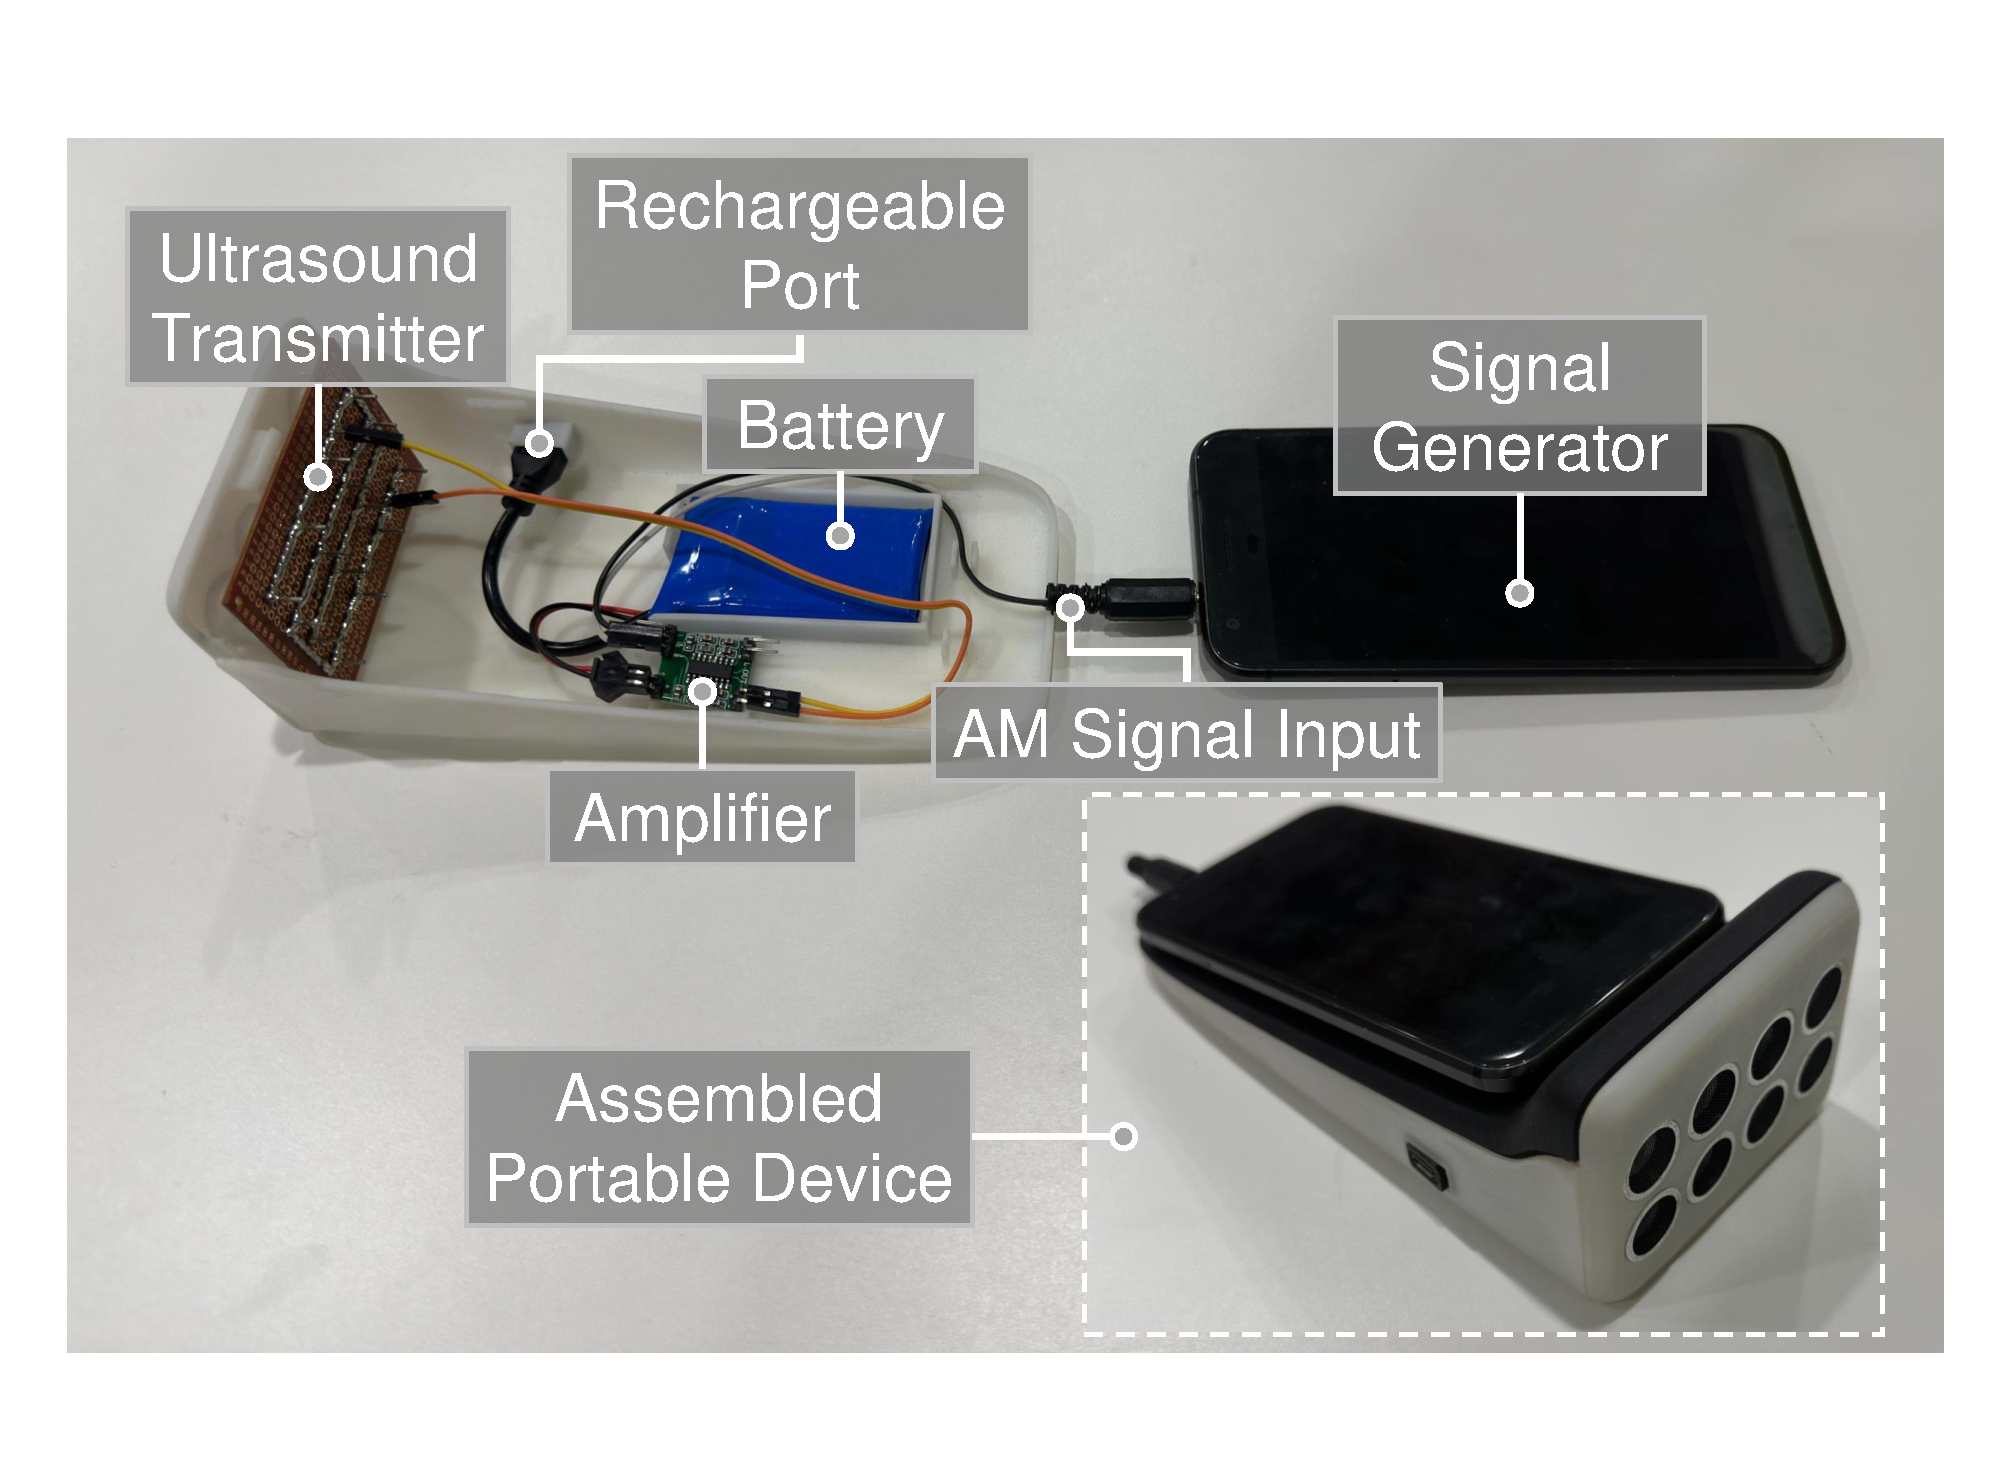
\includegraphics[width=1.06\textwidth]{portable_device.pdf} % height=0.765\linewidth
    	\end{minipage}
        }\hfill
	\subfigure[Off-the-shelf Loudspeaker]{   %第一张子图
	\begin{minipage}[t]{0.22\textwidth}
		\centering
            % \hspace{-0.1\linewidth}
		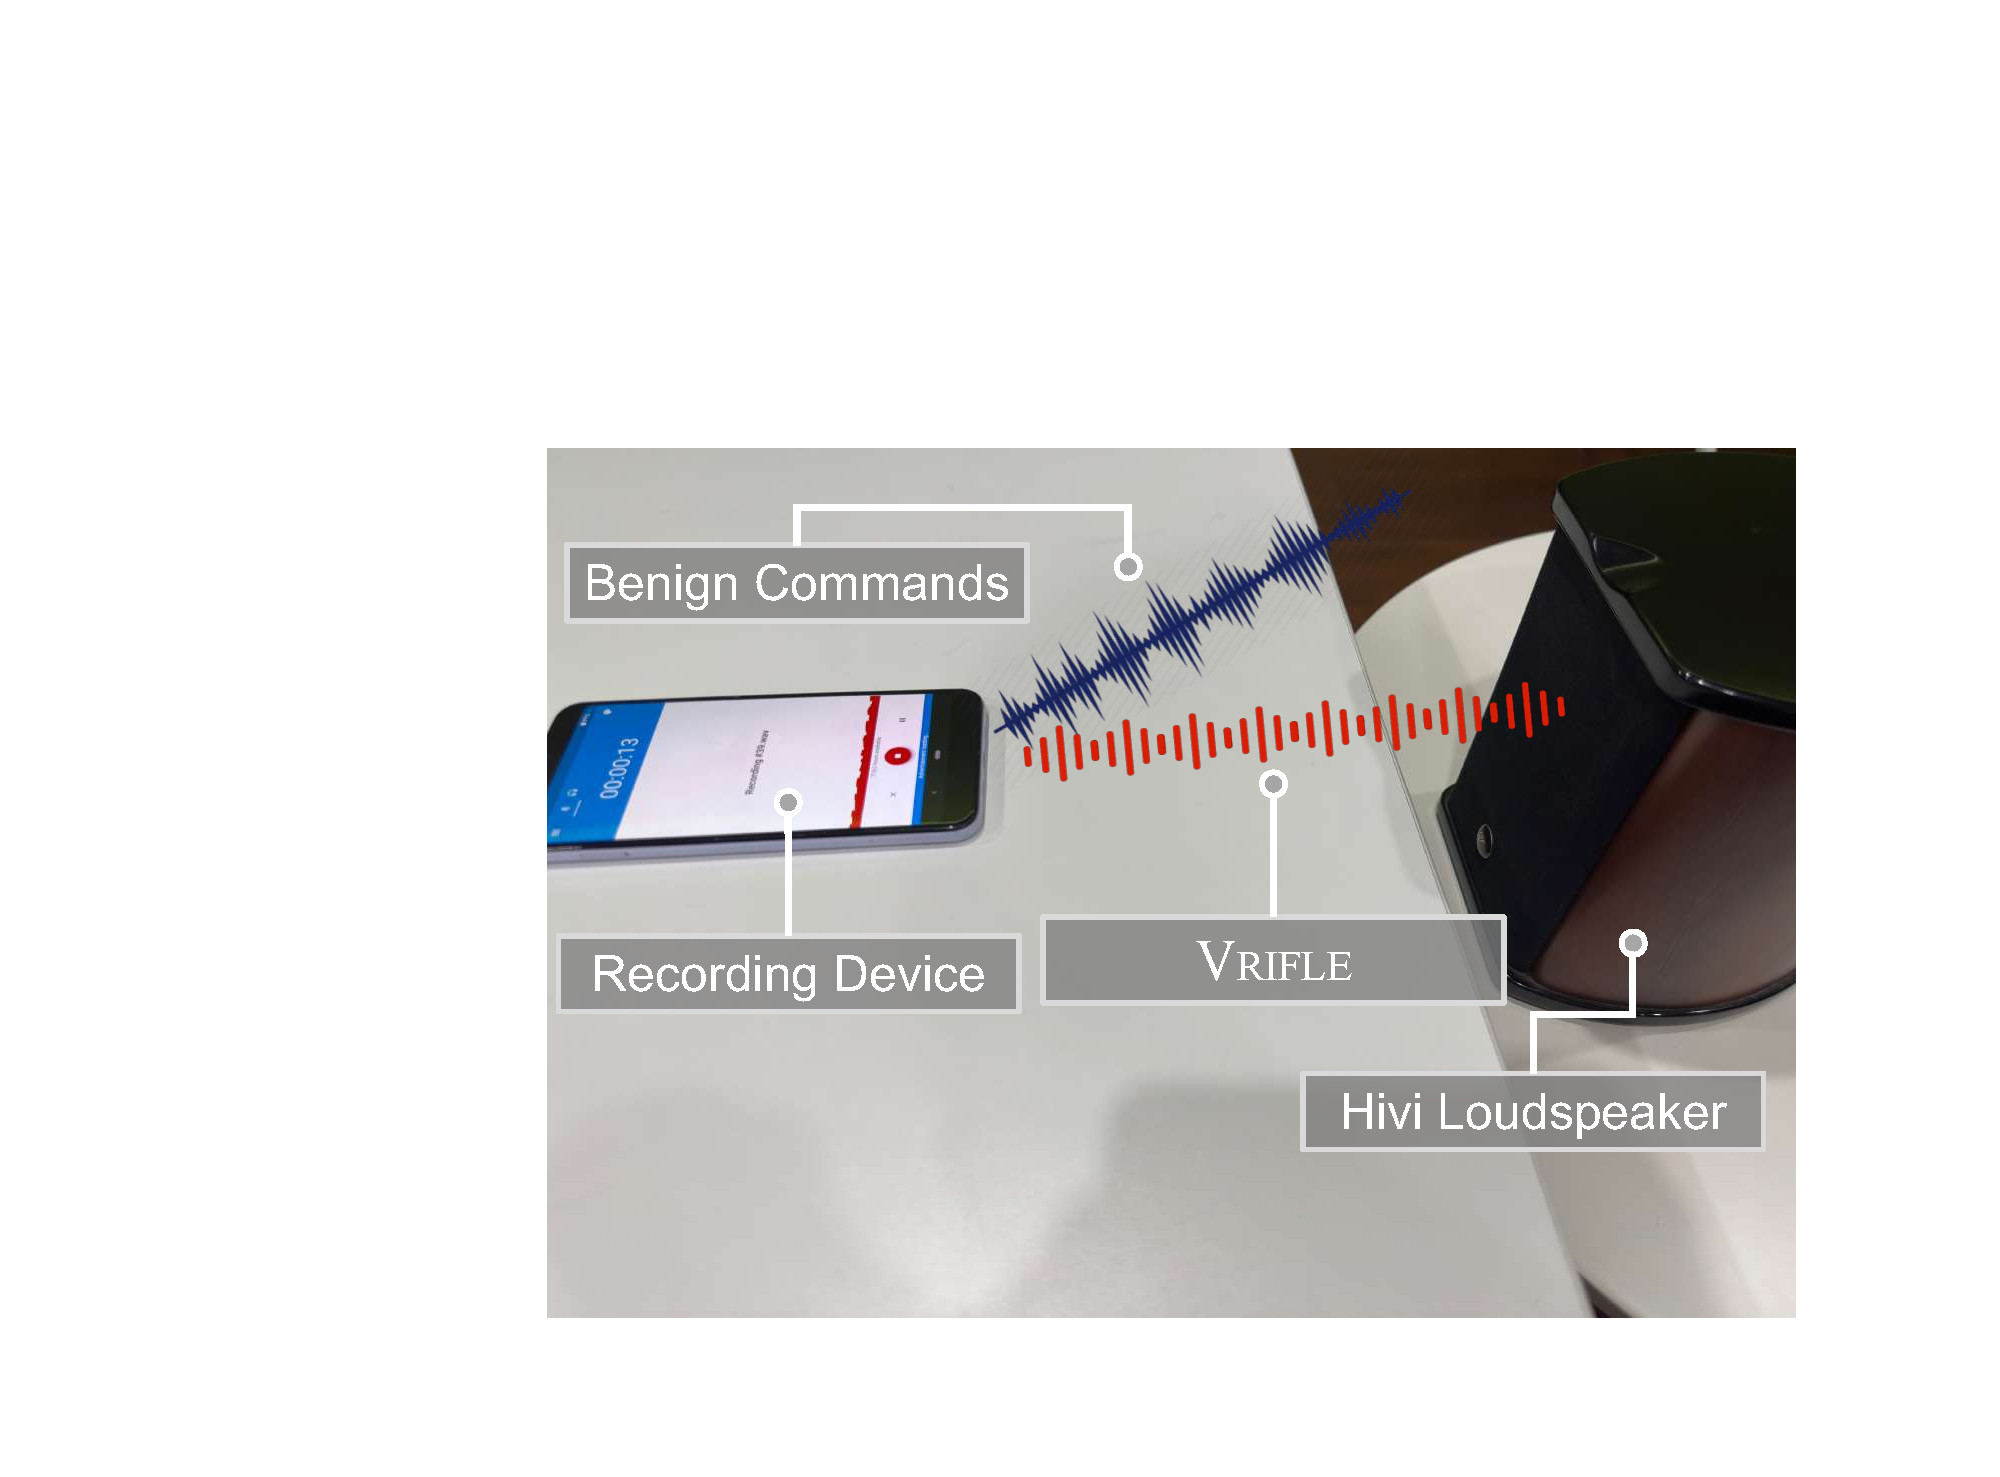
\includegraphics[width=1.03\textwidth]{hivi_speaker4.pdf} 
	\end{minipage}
	}
	\caption{Two additional attack forms of \alias.}    %大图名称
	\label{fig:portable_device}    %图片引用标记
	\vspace{-10pt}
\end{figure}


\begin{figure}[t]
	\centering  %居中
        \subfigure[Portable Device]{   %第一张子图
    	\begin{minipage}[t]{0.23\textwidth}
    		\centering
    		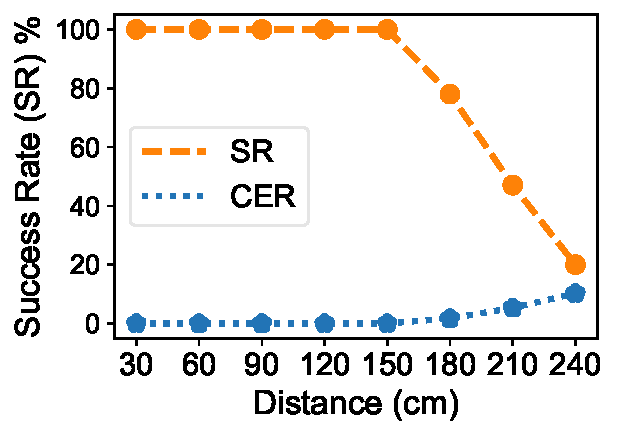
\includegraphics[width=1\textwidth]{eval_portable.pdf} % height=0.765\linewidth
    	\end{minipage}
        }\hfill
	\subfigure[Off-the-shelf Loudspeaker]{   %第一张子图
	\begin{minipage}[t]{0.207\textwidth}
		\centering
            % \hspace{-0.1\linewidth}
		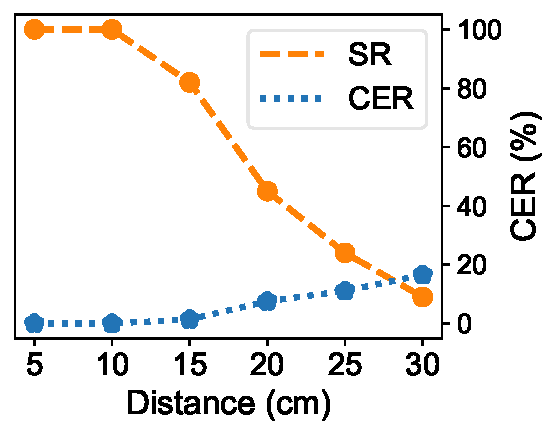
\includegraphics[width=1\textwidth]{eval_hivi.pdf} 
	\end{minipage}
	}
	\caption{\alias's performance at different distance with the portable device and off-the-shelf loudspeaker.}    %大图名称
	\label{fig:eval_portable_hivi}    %图片引用标记
	\vspace{-10pt}
\end{figure}

\section{Anti-defense Experiment}
In this section, we validate whether \alias can resist 6 kinds of representative defenses, involving audio pre-processing methods and inaudible attack detection. We consider two types of adversaries: 1) \emph{Naive Adversary}: The naive adversary creates \alias based on the undefended model to attack the defended model. 2) \emph{Adaptive Adversary}: This adversary has full knowledge of the defense mechanisms and applies customized strategies to craft \alias.

% \subsection{Against Audio Pre-processing Defense Methods} 
\textbf{Against Audio Pre-processing Defense Methods.} 
Referring to previous works~\cite{hussain2021waveguard,deng2022fencesitter,li2020advpulse,yuan2018commandersong} that present a series of audio pre-processing methods against audio adversarial example attacks, we examine the robustness of \alias using 5 representative defenses: \textit{(1) Quantization}: converting the audio sampling value from a 16-bit signed integer to an 8-bit precision, which reduces the sampling range from [-32,768$\sim$32,767] to [-128$\sim$127]. Notably, this introduces distortion and noise due to the small range of values at 8-bit precision. \textit{(2) Voice Activity Detection (VAD)}: removing segments of audio that are less than -15~dB, where its maximum energy is normalized to 0~dB. \textit{(3) Opus Compression Codec}: coding and compressing audio with flexible bit rate and low latency are widely used in real-time communication, particularly VoIP and online meetings. We set the default compression level as 5 according to \cite{torch_codec}. \textit{(4) Band-pass Filter}: filtering the input signal with given cut-off frequencies, e.g., 50$\sim$7000 Hz. \textit{(5) Down-sampling}: reducing the audio to a given rate, e.g., rate=0.4 means down-sampling a 16 kHz audio to 6.4 kHz, and then recovering it to the required sampling rate of targeted ASRs (generally 16/48~kHz).

We obtain the attack success rate (successfully altering the tested speech into the targeted command ``open the door''), attack CER, and benign CER (derived between the DeepSpeech recognized and ground-truth transcription) at 99.49\%, 0.15\%, 11.23\%, respectively, when the model is undefended.
The results are listed in Tab.~\ref{tab:definitive}, \ref{tab:bandpass}, \ref{tab:squeezing}. We observe that quantization, VAD, and Opus compression barely affect the attack success rate (all$\ge$95.93\%) in Tab.~\ref{tab:definitive}. Particularly, VAD significantly rises benign CER from 11.23\% to 23.58\%, while failing to lower our attack performance. Tab.~\ref{tab:bandpass} and \ref{tab:squeezing} demonstrate that naive \alias can maintain relatively effective even when facing a 50$\sim$4000 band-pass filter or being down-sampled to 8 kHz (rate=0.5). However, the attack performance degrades as the bandwidth or the down-sampling rate gets further lower. Note that we do not evaluate extreme cases, such as band-pass: less than 50$\sim$2000 Hz or down-sampling rate: smaller than 0.3, since they have severely affected the model's ability to transcribe benign speech commands with unacceptable CERs over 45\%. After the adaptive adversary integrates the band-pass filtering operation during optimization, the attack performance increase significantly, especially the success rate and attack CER reach 78.88\% and 5.34\%, respectively, even under 50$\sim$3000 Hz band-pass filtering. Similarly, the adaptive adversary can realize an 81.42\% success rate and 4.38\% CER against a down-sampling rate=0.4.


% 这里主要体现随着defense中down-sample 和 squeezing的改变,会导致攻击成功率下降,但是值得注意的是正常音频的识别也会受到很大影响。
\begin{table}[t]
\footnotesize
\centering
\renewcommand\arraystretch{0.8} 
\setlength\tabcolsep{2.8pt}
\caption{Three defenses}
\begin{tabular}{c|c|c|c|c}
\toprule[1pt]
\multicolumn{1}{c|}{\textbf{(\%) Method}} & \multicolumn{1}{c|}{\textbf{Undefended}} & \textbf{Quantization} & \textbf{VAD}   & \textbf{Opus Compress} \\ \midrule[0.8pt]
\multicolumn{1}{c|}{Success Rate}                      & \textbf{99.49}                           & 97.96        & 99.49 & 95.93         \\ \midrule
\multicolumn{1}{c|}{Attack CER}                      & \textbf{0.1}                            & 0.28         & 0.1  & 0.84          \\ \midrule
\multicolumn{1}{c|}{Benign CER }                     & \textbf{11.23}                           & 13.43        & 23.58 & 12.37         \\ \bottomrule[1pt]
\end{tabular}
\label{tab:definitive}
\vspace{-5pt}
\end{table}

\begin{table}[t]
\footnotesize
\centering
\renewcommand\arraystretch{0.8} 
\setlength\tabcolsep{1pt}
\caption{Defense with band-pass filter}
\begin{tabular}{cc|c|c|c|c|c}
\toprule[1pt]
\multicolumn{2}{c|}{\textbf{(\%) Band-pass (Hz)}}                                                                               & \multicolumn{1}{l|}{\textbf{50$\sim$7000}} & \multicolumn{1}{c|}{\textbf{50$\sim$6000}} & \multicolumn{1}{l|}{\textbf{50$\sim$5000}} & \multicolumn{1}{l|}{\textbf{50$\sim$4000}} & \multicolumn{1}{l}{\textbf{50$\sim$3000}} \\ \midrule[0.8pt]
\multicolumn{1}{c|}{\multirow{2}{*}{\multirow{2}{*}{\begin{tabular}[c]{@{}c@{}}\emph{Naive}\\ \emph{Adversary}\end{tabular}}}}    & Success Rate & 97.96                             & 96.95                             & 95.67                             & 75.57                             & 12.47                            \\ \cmidrule{2-7} 
\multicolumn{1}{c|}{}                                                                              & Attack CER   & 0.28                              & 0.53                              & 0.80                              & 6.43                             & 35.01                            \\ \midrule[0.8pt]
\multicolumn{1}{c|}{\multirow{2}{*}{\multirow{2}{*}{\begin{tabular}[c]{@{}c@{}}\emph{Adaptive}\\ 
\emph{Adversary}\end{tabular}}}} & Success Rate & 99.75                             & 99.24                            & 97.20                             & 91.60                             & 78.88                            \\ \cmidrule{2-7} 
\multicolumn{1}{c|}{}                                                                              & Attack CER   & 0.05                              & 0.14                              & 0.41                              & 1.64                              & 5.34                            \\ \midrule[0.8pt]
\multicolumn{2}{c|}{Benign CER}                                                                                   & 11.63                             & 13.60                             & 19.27                             & 28.83                             & 41.06                            \\ \bottomrule[1pt]
\end{tabular}
\label{tab:bandpass}
\vspace{-5pt}
\end{table}

\begin{table}[t]
\footnotesize
\centering
\renewcommand\arraystretch{0.8} 
\setlength\tabcolsep{2.8pt}
\caption{Defense with down-sampling}
\begin{tabular}{cc|c|c|c|c|c|c}
\toprule[1pt]
\multicolumn{2}{c|}{\textbf{(\%) Down-sample (rate)}}                                                                               & \multicolumn{1}{c|}{\textbf{0.9}} & \multicolumn{1}{c|}{\textbf{0.8}} & \multicolumn{1}{c|}{\textbf{0.7}} & \multicolumn{1}{c|}{\textbf{0.6}} & \multicolumn{1}{c|}{\textbf{0.5}} & \multicolumn{1}{c}{\textbf{0.4}}  \\ \midrule[0.8pt]
\multicolumn{1}{c|}{\multirow{2}{*}{\multirow{2}{*}{\begin{tabular}[c]{@{}c@{}}\emph{Naive}\\ \emph{Adversary}\end{tabular}}}}    & Success Rate & 98.98                             & 98.22                             & 94.91                             & 88.04                             & 69.47  & 19.34                            \\ \cmidrule{2-8} 
\multicolumn{1}{c|}{}                                                                              & Attack CER   & 0.20                              & 0.27                             & 1.00                              & 2.58                              & 8.35    &  30.23                            \\ \midrule[0.8pt]
\multicolumn{1}{c|}{\multirow{2}{*}{\multirow{2}{*}{\begin{tabular}[c]{@{}c@{}}\emph{Adaptive}\\ 
\emph{Adversary}\end{tabular}}}} & Success Rate & 99.24                             & 98.22                             & 96.69                             & 95.42                             & 89.06  & 81.42                            \\ \cmidrule{2-8} 
\multicolumn{1}{c|}{}                                                                              & Attack CER   & 0.14                              & 0.27                             & 0.57                              & 0.87                              & 2.25    &  4.38                            \\ \midrule[0.8pt]
\multicolumn{2}{c|}{Benign CER}                                                                                   & 11.51                             & 12.11                             & 14.93                             & 19.80                             & 23.99   &  35.04                            \\ \bottomrule[1pt]
\end{tabular}
\label{tab:squeezing}
\end{table}

% \subsection{Against Inaudible Attack Detection Method}

\begin{figure}[t]
    \centering
    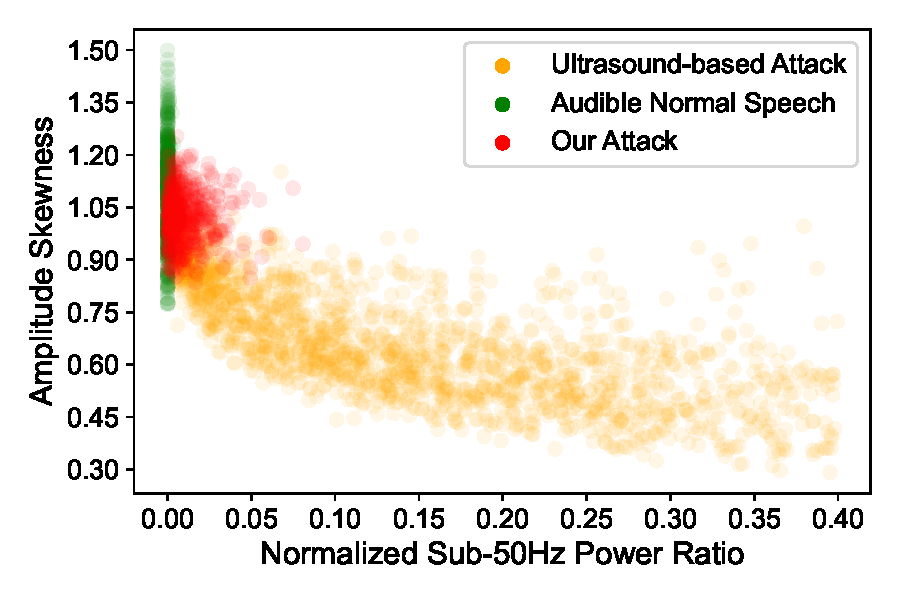
\includegraphics[width=0.34\textwidth]{detect_compare.pdf}
    \caption{Two significant feature dimensions extracted from three classes of audio samples by LipRead (800 samples/class).}
    \label{fig:detect_compare}
    \vspace{-10pt}
\end{figure}

\textbf{Against Inaudible Attack Detection Method.} 
Given that \alias utilizes ultrasound-based modulation mechanisms, prior inaudible attack detection methods are expected to distinguish such an attack well from benign speech. We reproduce the representative software-based method: LipRead~\cite{roy2018inaudible}, strictly following its instruction, which extracts and analyzes three features of speech samples: power in sub-50Hz, correlation coefficient (between the fundamental and harmonic components), and amplitude skew. 
We use the LipRead classifier to detect \alias samples crafted under the naive adversary setting and collected at different distances \& angles; then obtain a detection accuracy down to 45.07\%. Fig.~\ref{fig:detect_compare} visualizes three types of audio samples in two significant feature dimensions. \alias presents compact skewness around 1.0 due to its symmetrical waveform, whose distribution is closer to the normal, while ultrasound-based attacks appear more shift toward 0.30 and greater power in sub-50Hz. Low-frequency power aggregation is still inevitable in our attack due to nonlinear demodulation~\cite{roy2018inaudible}. Moreover, naive \alias appears low correlation coefficient compared to the traditional attacks, as its perturbations (see Fig.~\ref{fig:design_overview}\&\ref{fig:design_attack}) barely present normal speech properties such as fundamental and harmonic frequencies. 
Overall, the inherent difference between \alias and traditional ultrasound-based attacks makes it probably compromise LipRead.
Furthermore, the adaptive adversary extracts three features during the perturbation generation and constrains them close to the normal samples, further reducing the accuracy of LipRead detecting our attack to 30.55\%.